\documentclass{article}
\usepackage{amsmath}
\usepackage{CJKutf8}
\usepackage{minted}
\usepackage{graphicx}

\title{Project Report of COMP130004}
\author{Fudanyrd}
\date{December, 2023}

\begin{document}
\begin{CJK*}{UTF8}{gbsn}
\maketitle
\par Github link to this Proj: http://github.com/Fudanyrd/COMP130004.git

\section{基础数据结构}

\paragraph{Matrix}
 考虑到用户之间的朋友关系是对称的,所以相应图的邻接矩阵表示是对称矩阵,可以用
上三角阵压缩存储.
\paragraph{User}
 每个用户都有属性id(身份标识码),rowNum(在邻接矩阵中存储的行号),所以用一个结构体封装.
\paragraph{HashTable}
除留余数法为散列函数,用开散列法解决冲突的散列表,关键码为用户id,可以实现在$O(1)$时间内
根据用户身份标识码查找在邻接矩阵中所在行号.
\paragraph{UserList}
建立上述散列表和一个行号为关键码的向量(由于行号不重复,无需考虑堆积),可以在$O(1)$时间内
实现行号和用户标识码的一一对应.
\paragraph{Relationship}
接口类,执行handout中提及的所有功能.
\paragraph{tuple}
在查找用户的间接朋友时有用,可以存储用户身份识别码和层级,层级为2者即为间接用户.
\par 程序结构如图所示:
\begin{figure}[H]
    \centering
    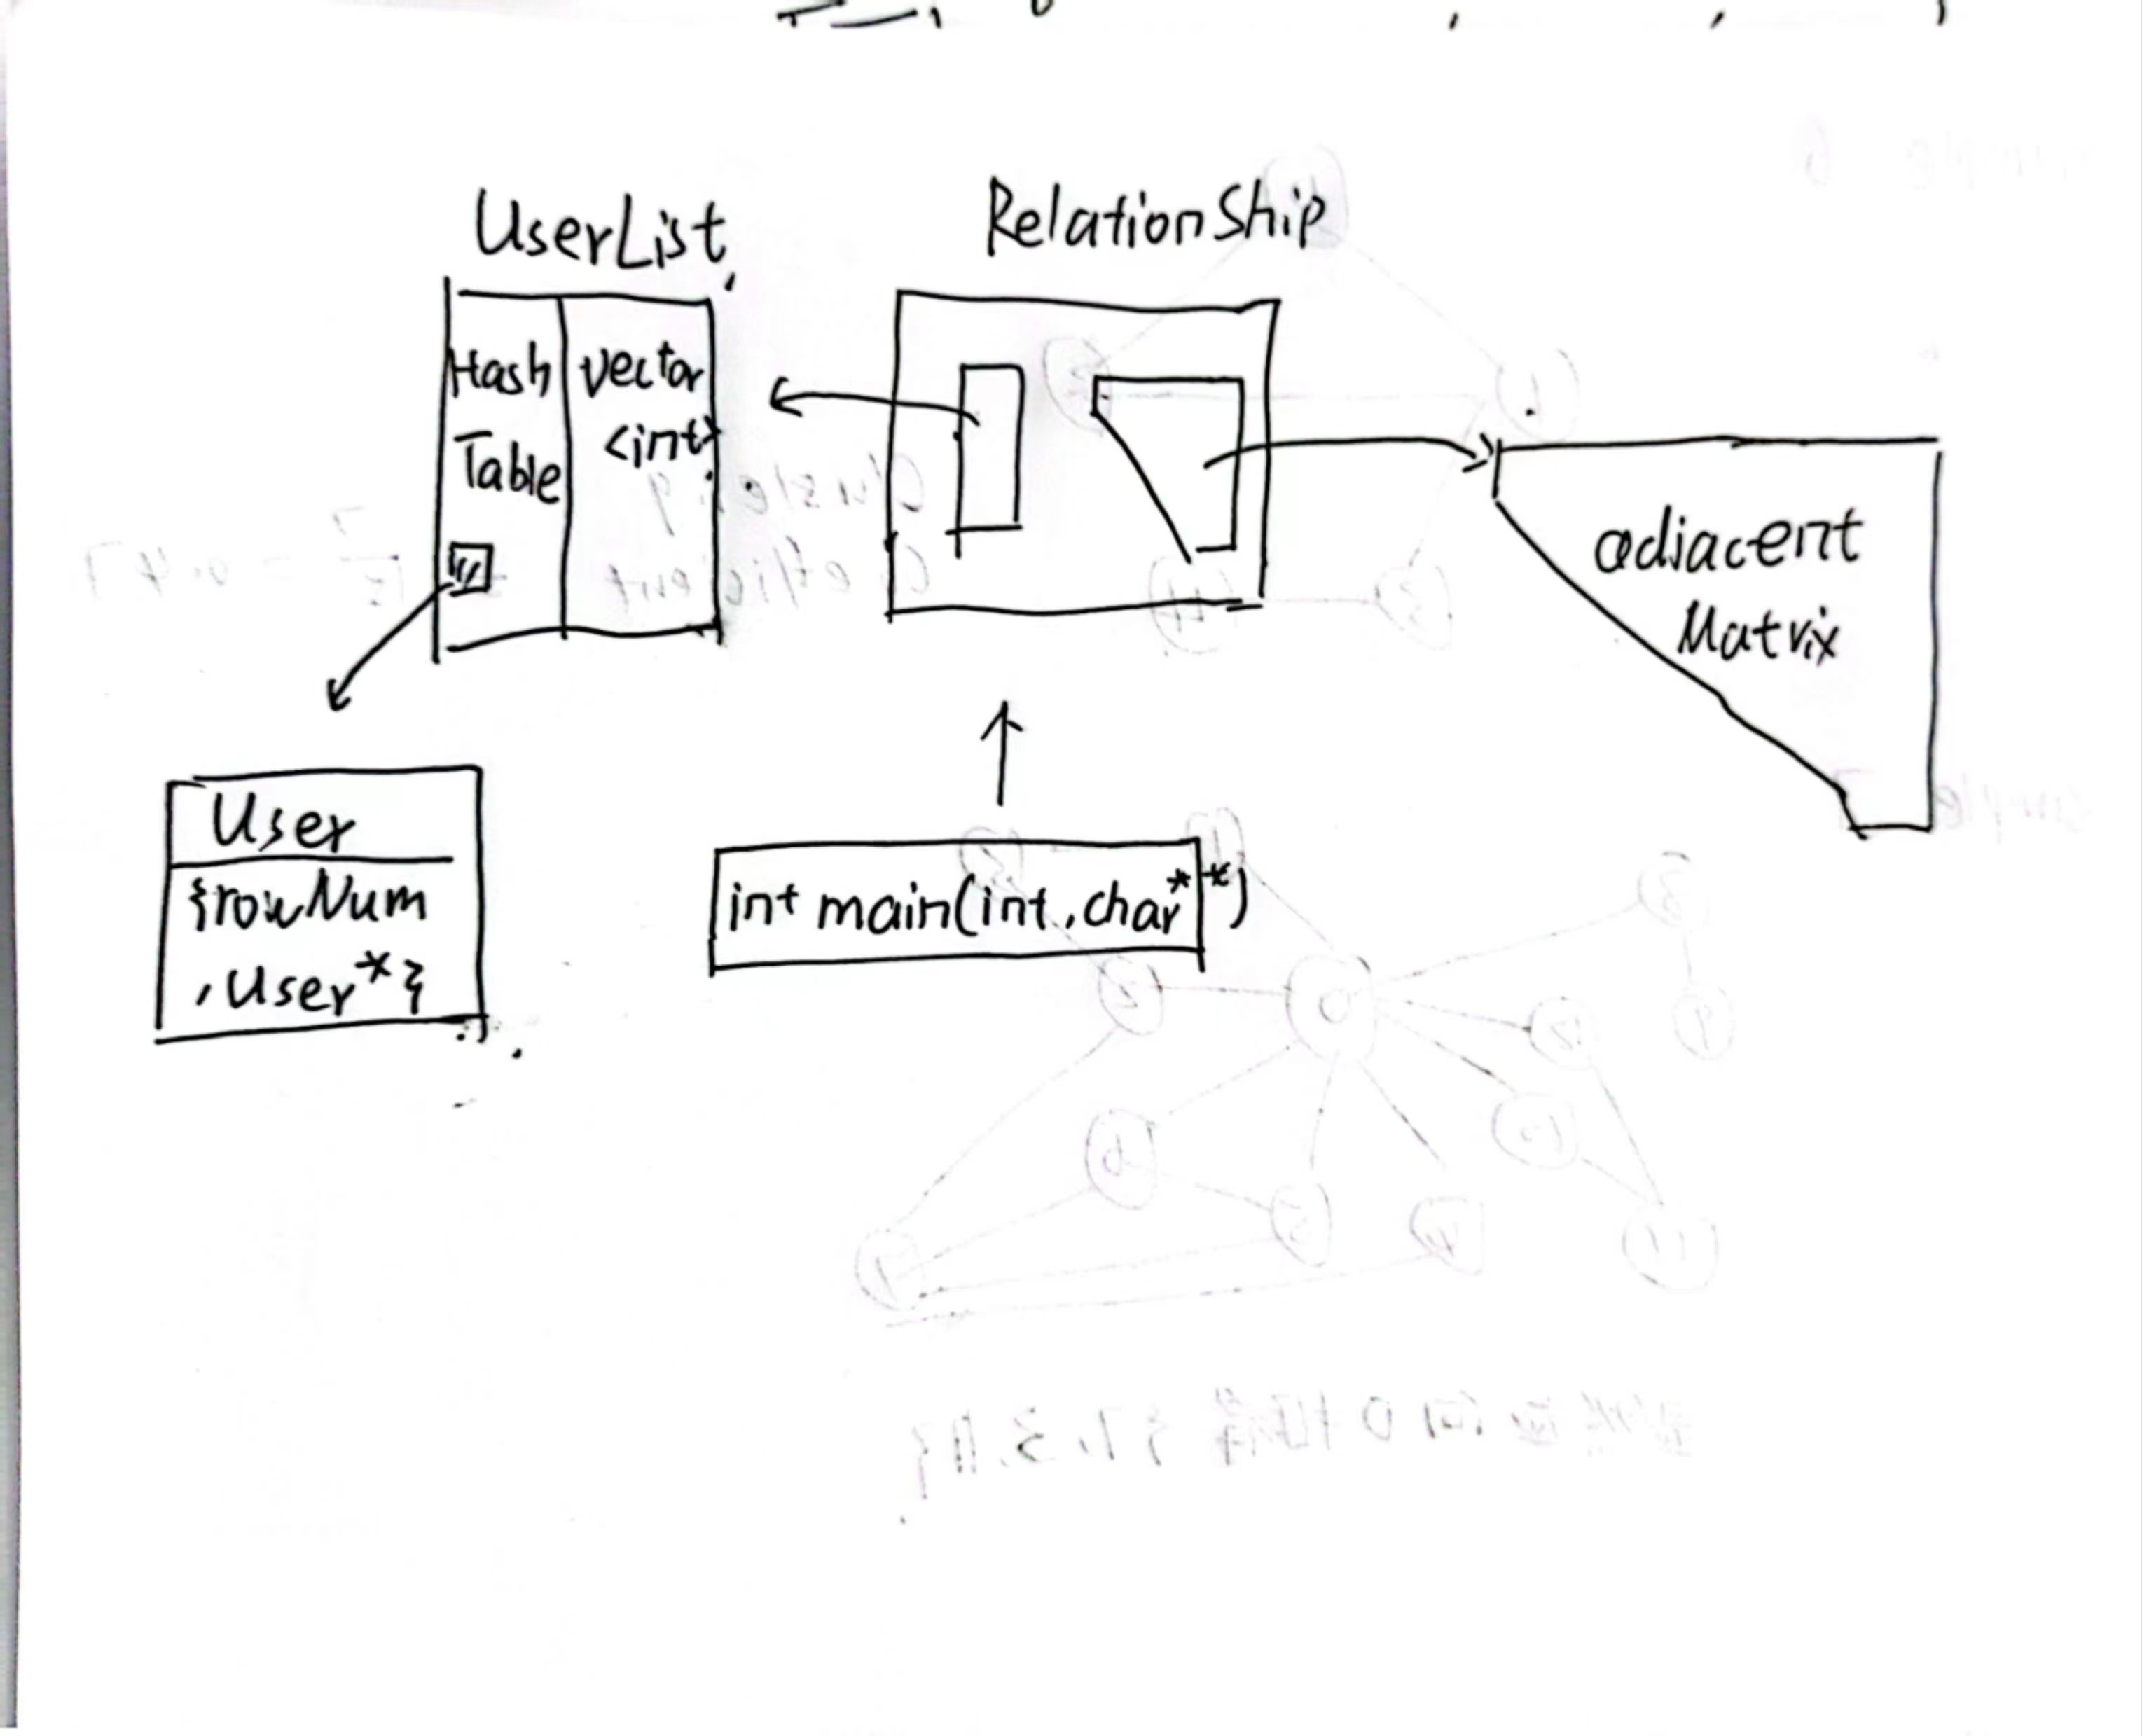
\includegraphics[width=0.75\textwidth]{explanation.jpg}
\end{figure}

\section{关键算法实现和复杂度分析}
\subsection{基本要求(1): 查询用户的直接和间接朋友数量}
\par 直接朋友数量即为邻接矩阵同一行中1的个数,扫描一遍即得,时间复杂度$O(N)$,空间复杂度$O(1)$.
\par 间接朋友数量需要广度优先搜索找出在同一连通分支中相对层级为2的用户个数,需要建立辅助存储空间标记用户是否
被访问过,找一个用户的邻居需要遍历邻接矩阵的某一行,故有时间复杂度$O(N^2)$,空间复杂度$O(N)$
同一连通分支中用户数量减去自身和直接朋友数量即为间接朋友数量.
\par 实现在"Relationship.hpp"中的numOfFriend和numOfSubFriend中.
\subsection{基本要求(2): 计算两个用户之间的最短社交距离}
\par 用广度优先搜索(可以保证是最小距离),找到所给用户或找遍一个连通分支为止,复杂度分析同上
: 时间复杂度$O(N^2)$,空间复杂度$O(N)$.
\par 实现在"Relationship.hpp"中的distanceOf中.
\subsection{基本要求(3): 超级连接者}
\par 暴力搜索,计算每个用户的朋友数,找最大值,总的时间复杂度$O(N^2)$,空间复杂度$O(N)$.
需要建立额外的存储空间是由于超级连接者可能不止一个,该算法找出所有的,通过向量返回.
\par 实现在"Relationship.hpp"中的superUsers函数中.
\subsection{高级要求(1): 高级网络分析算法}
\paragraph{Clustering Coefficient: } 根据handout中的方法先找出给定用户的所有朋友,再
分析这些朋友之间的连接情况,算法使用两层嵌套循环和向量为辅助存储空间,最坏情况下用户朋友个数的数量级为$O(N)$,
然后再逐个分析这些朋友之间的邻接关系,
故分析一个用户聚集系数的时间复杂度$O(N^2)$,空间复杂度$O(N)$,总的时间复杂度$O(N^3)$,空间复杂度$O(N^2)$.
\paragraph{朋友三角的数量: }依靠邻接矩阵的3次幂搞定,邻接矩阵的3次幂的trace(迹)是三角形个数的6倍.
一次矩阵乘法运算的时间复杂度$O(N^3)$,空间复杂度$O(N^2)$.
\subsection{高级要求(2): 用户推荐功能}
\par 对于给定的用户身份识别码,计算他与其他所有用户的共同朋友数(总时间复杂度$O(N*N)=O(N^2)$,总空间复杂度$O(1)$).
在从中选出3个共同朋友数最多的用户(时间复杂度$O(N)$,空间复杂度$O(N)$因为借助了辅助空间),故总的时间复杂度$O(N^2)$,
空间复杂度$O(N)$.

\section{运行结果}
\par 选用原始文档里的"sample.txt"去掉注释作为测试数据,在wsl下编译结果如下:
\begin{figure}[H]
    \centering
    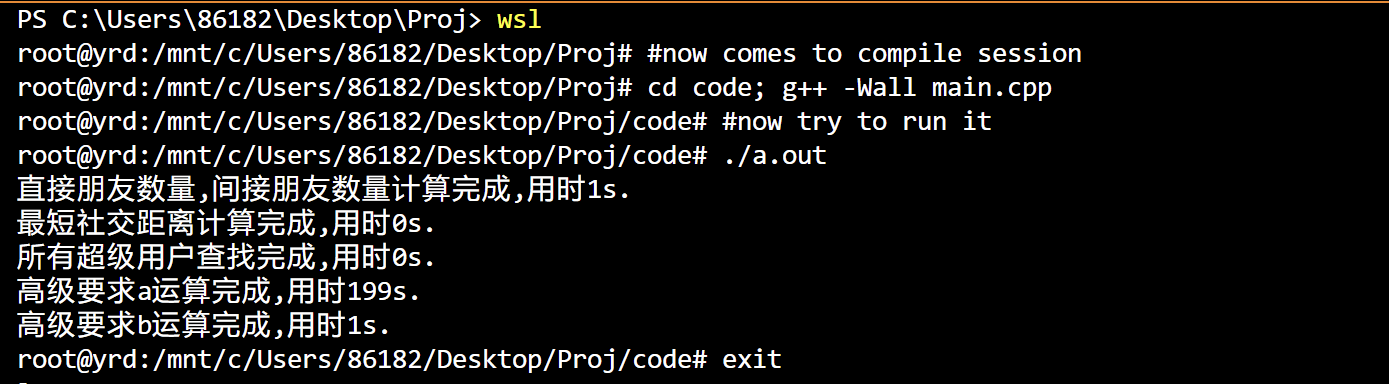
\includegraphics[width=0.75\textwidth]{compile.png}
\end{figure}
\par 运行结果如下:
\begin{figure}[H]
    \centering
    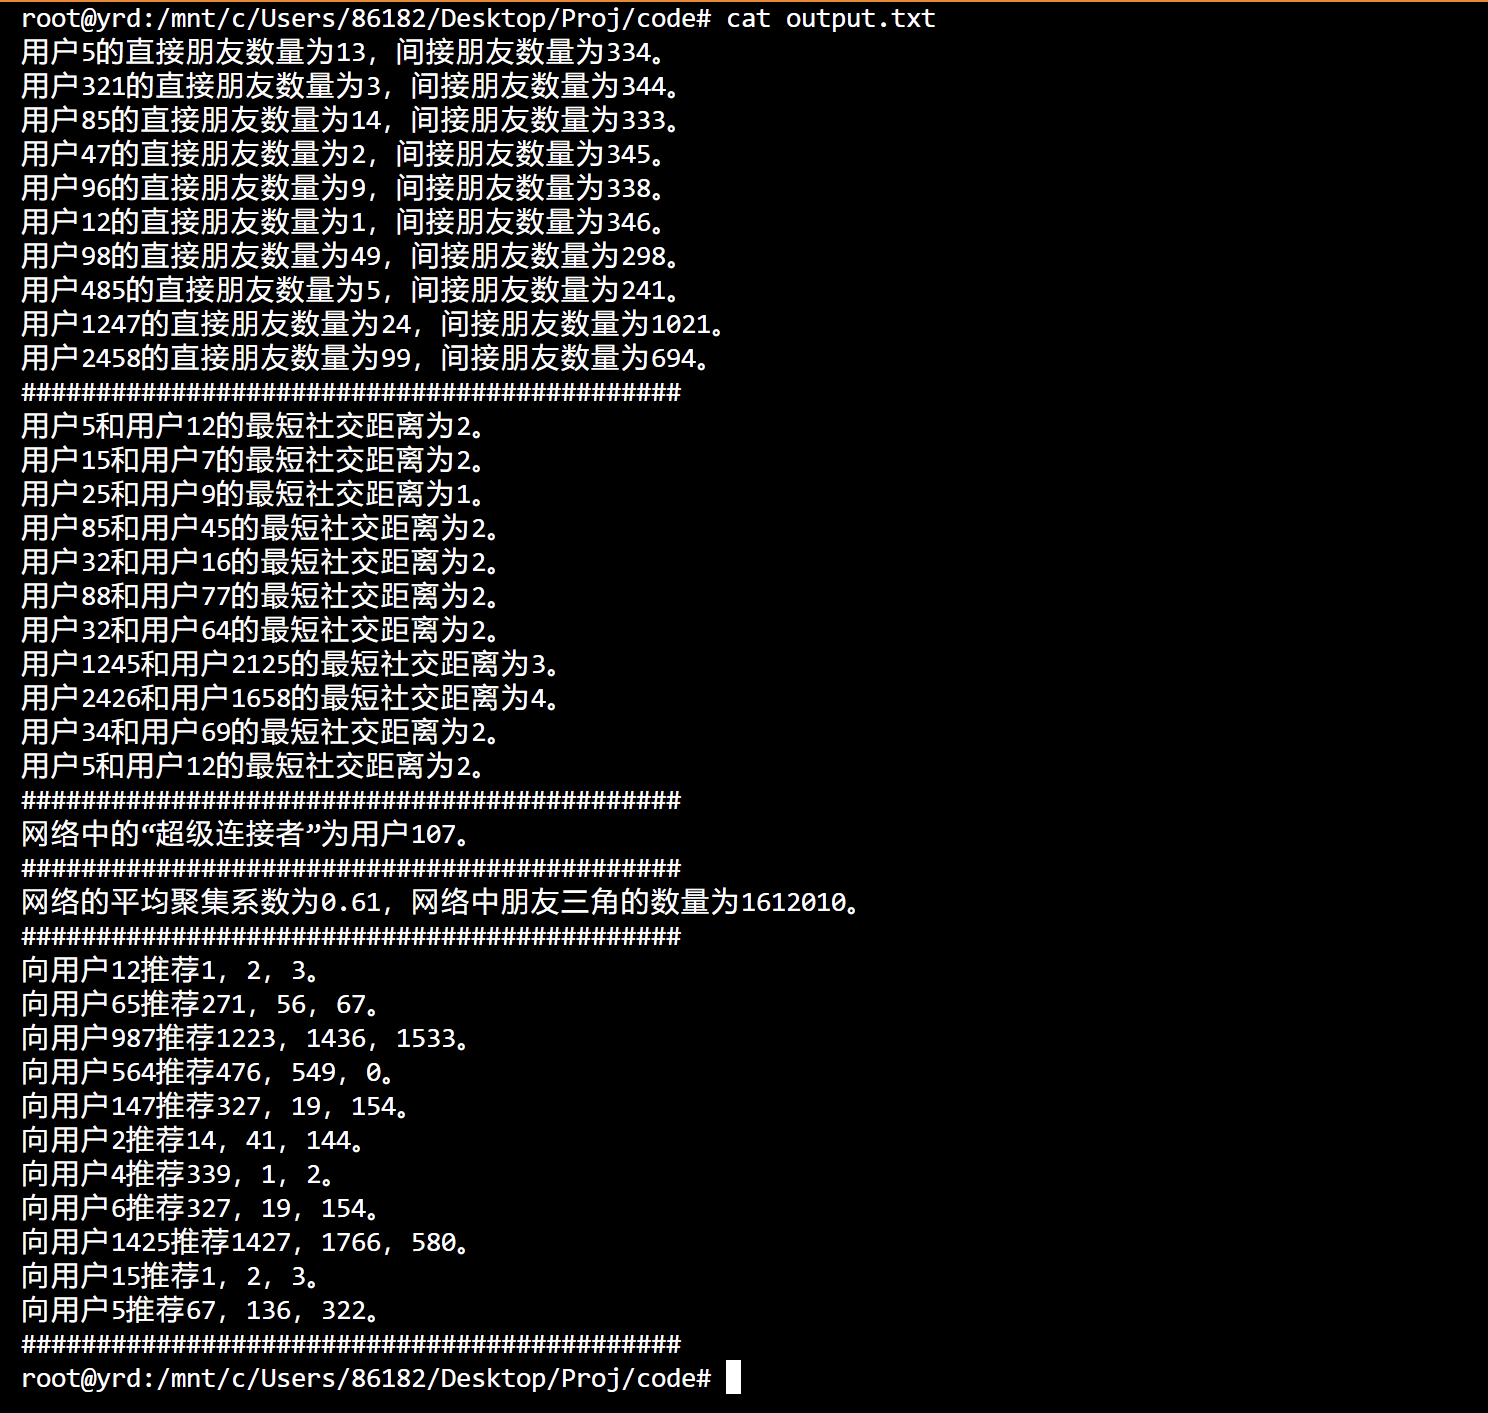
\includegraphics[width=1.0\textwidth]{run.png}
\end{figure}

\section{写在最后}
\par 本人在完成此次Proj的过程中未借助任何AI工具,没有从互联网和其他同学那里复制粘贴代码段.
\par 当然,希望尊敬的张老师以后能早一点 release Proj.(哭)

\end{CJK*}
\end{document}